\documentclass{article}
\usepackage{authblk}
\usepackage[T1]{fontenc}
\usepackage[utf8]{inputenc}
\usepackage{graphicx}
\usepackage{listings}
\usepackage{placeins}

\title{Recursion, Game Trees and Classes - Making an unbeatable algorithm.}

\author[]{Tushar Rakheja}
\author[]{Shibjash Dutt}
\author[]{Hanit Banga}

\affil[]{\texttt{Instructors @ Endofline Computer Club}}

\renewcommand\Authands{ and }

\date{August 2015}

\begin{document}

\maketitle

\section{Introduction}

In the last session, we talked about functions. We'll start this session by talking about recursive functions. These are functions that refer to themselves, in order to compute what they're meant to. We'll discuss the theory, some classic examples, and some interesting questions that are recursive in nature. \\

\noindent After that, we'll take a slight detour into programming and learn about lists in Python. A list is a data structure \cite{DSinPres_Slide} that stores elements sequentially.\\

\noindent Once we're done with lists, we'll come back to Tic-Tac-Toe, but this time we'll look at it with little to no code. We'll then introduce the tree data structure, and the class programming construct. Finally, we'll put all of it together, and assemble the Earth's Mightiest Zeros. 

\section{Recursive Functions}

\noindent So far, we've seen that a function is just a set of instructions in a program that can be called to perform the same set of instructions on different \textit{arguments}. Even though this seems like a simple thing, a cleverly designed function can perform awefully complex computations depending upon the argument. It's a necessary tool for a programmer. You'll see. Let's see what we mean by introducting the concept of \textit{recursive functions}. \\

\noindent Recursive functions, in many ways, are just like normal functions. They take in some arguments and perform a series of instructions. However, there's one key difference - one of these intructions in a recursive function is a call to itself. \\

\noindent "... wait, what?" Yeah, we know. A recursive function calls itself, you read it right. And when it calls itself, it again calls itself as a part of the call (since it performs the same series of instructions - it's the same function after all). Doesn't that sound like an infinite loop? It may, but it isn't of course. Each time a recursive function calls itself, something changes, which eventually stops this otherwise endless self-calls - \underline{the argument}. \\

\noindent A recursive function has something called a \underline{base case} or an \underline{end condition}, that depends upon the argument. When the argument attains a certain value, the base case is triggered, and the function doesn't call itself again. (As you may have guessed, this base case is checked using an if\{ \} block) Before saying anything else, let's look at an example - let's write a function to multiply two integers, $a$ and $b$. \\

\noindent \underline{\textit{Version 1: Non-recursive}} 
\begin{lstlisting}[language=Python]

def mult(a, b):     
    return a*b 
    
\end{lstlisting} 
\vspace{5mm}

\noindent \underline{\textit{Version 2: Recursive}} 
\begin{lstlisting}[language=Python]

def mult(a, b):
    if (b == 0):
        return 0
    else:
        return a + mult(a, b-1)
        
\end{lstlisting}
\vspace{5mm}

\noindent This example was terribly trivial (especially Version 1, to the point of being unnecessary). But, do you see how Version 2 works? On the next page there's a visualization with $a = 3$ and $b = 4$. Follow the small black arrows first, paying attention only to things in black. Once you reach the end, follow the red arrows back up along with the explanation. Each function call looks like this: 

\FloatBarrier
\begin{figure}
    \centering
    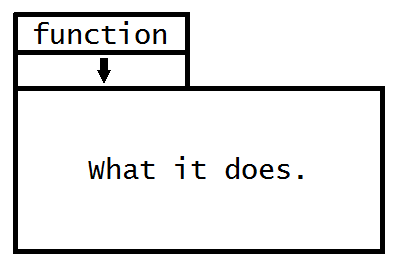
\includegraphics[scale=0.5]{SampleFunction}
    \caption{Sample Function.}
    \label{SampleFunction}
\end{figure}
\newpage 

\begin{figure}
    \centering
    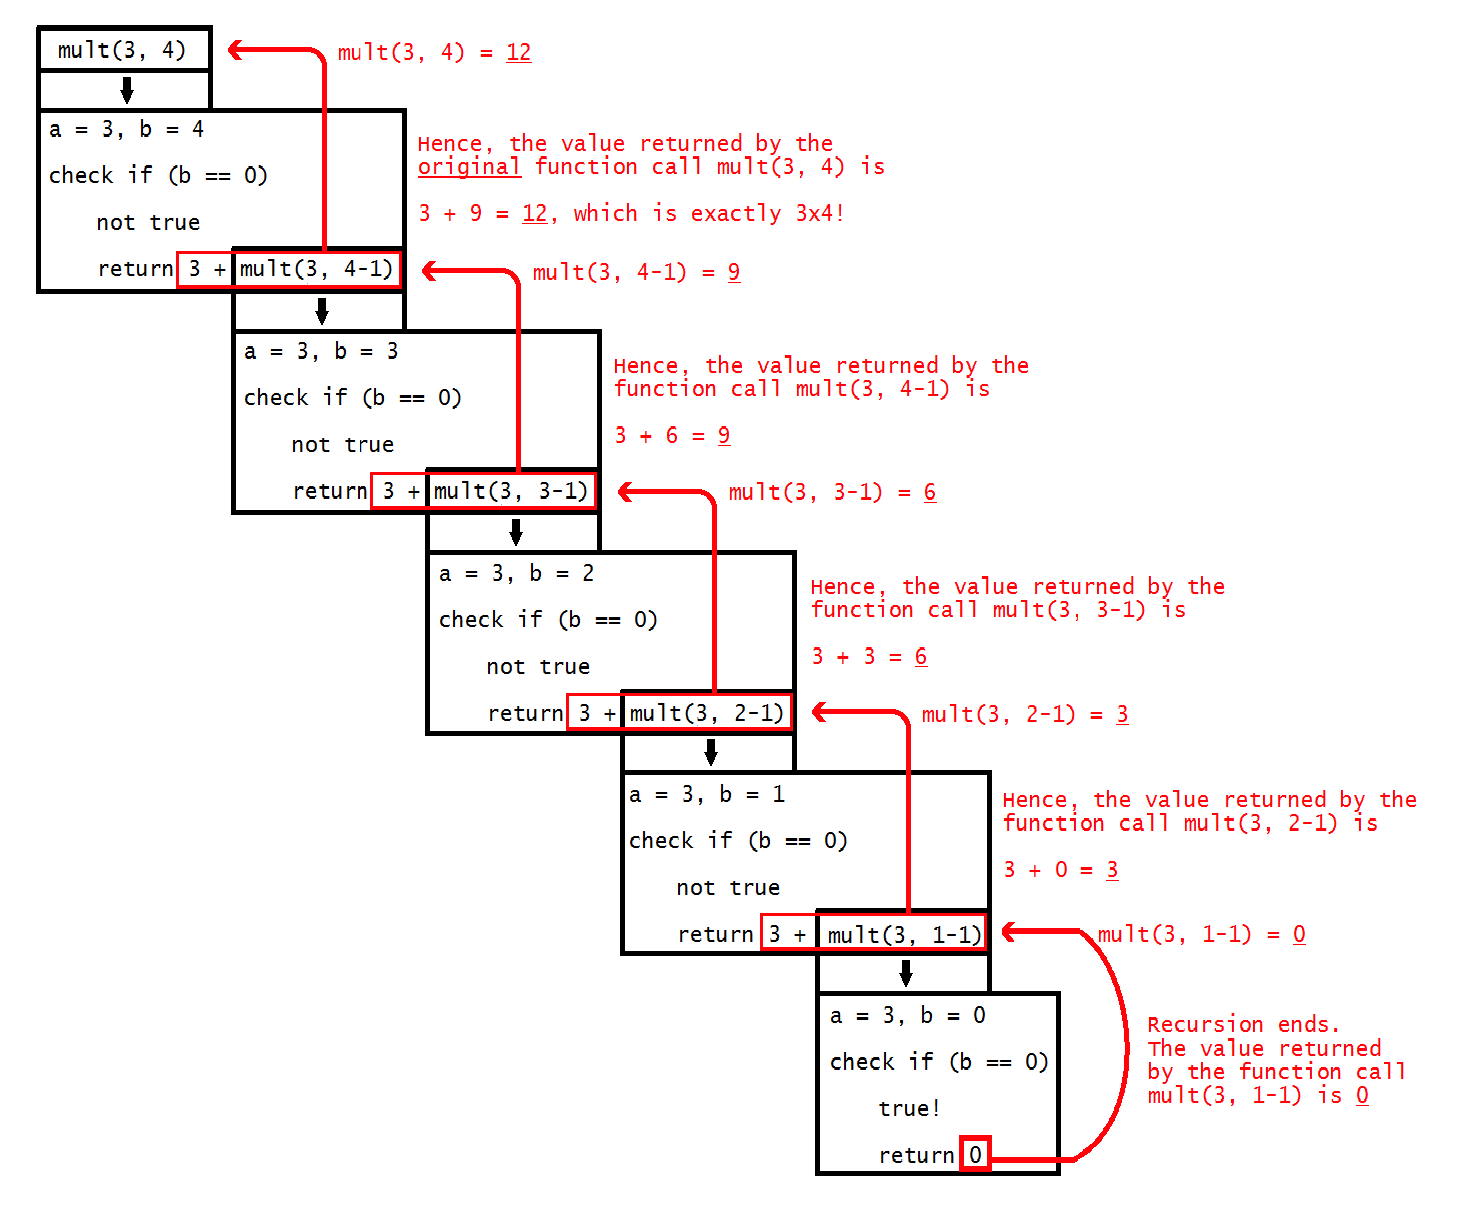
\includegraphics[scale=0.415]{Recursion}
    \caption{Visualizing mult(3, 4), Version 2.}
    \label{Recursion}
\end{figure}
\FloatBarrier

\section{Lists}

\section{Trees}

\section{Game states} 

So far, we've looked at various tools, like functions, recursion and lists,
which will help us in our analysis of the game. Let us now start working with
a more concrete idea, that of \textit{game states}. \\

\noindent Imagine a game of Tic-Tac-Toe played between Alice and Bob. Alice is playing crosses (X) and Bob is playing zeros (O). \\

\noindent Here is an example of how such a game might proceed, if Alice plays first:

\begin{center}
    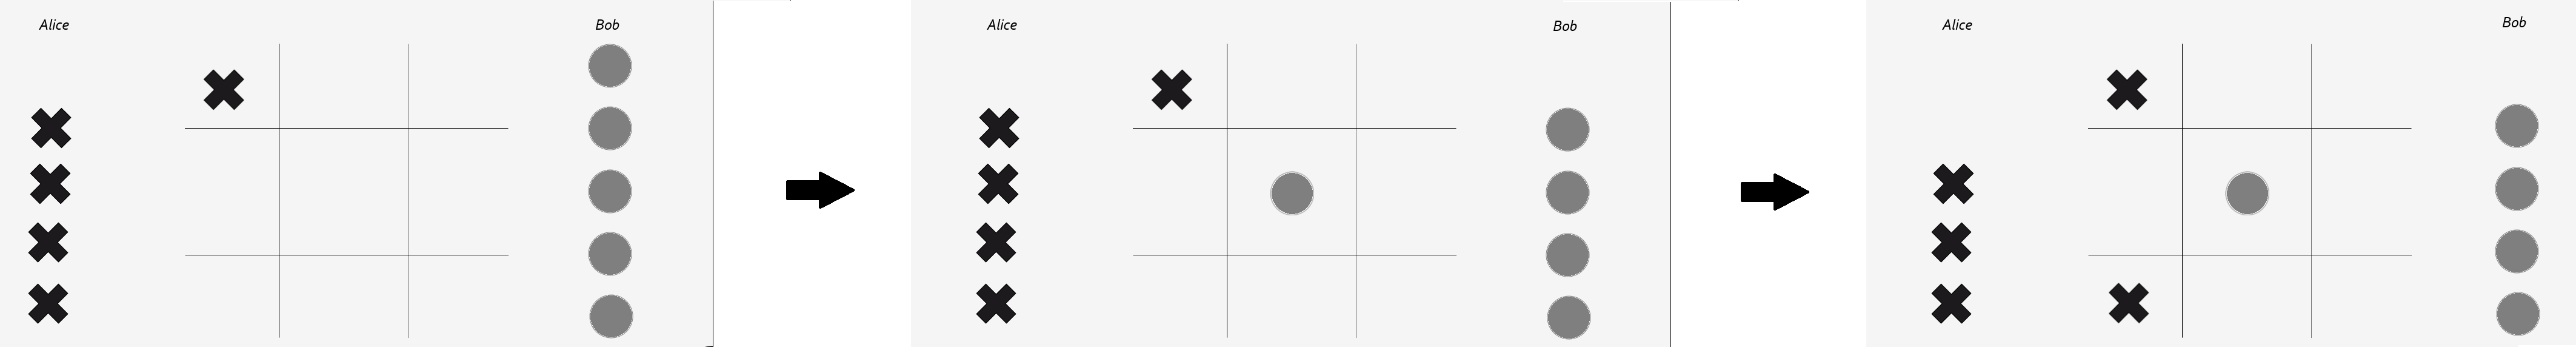
\includegraphics[scale=0.11]{AliceVBob}
\end{center}

\noindent And so on. \\

\noindent A \textit{game state} is, predictably, the \textit{state} or the configuration of the game, at some particular time. As far as Tic-Tac-Toe is concerned, we could define the game state to be the "contents" of the board and their respective locations at some time \textit{t}. \\

\noindent Informally, the game state is a "snapshot" or a "photograph" of the board at some time. A simple concept, but why's it useful? Let's see. 

\section{Classes}

\section{Putting it all together}

\subsection{Game Trees}

\subsection{Relating game states to game trees}

\begin{thebibliography}{9}
\bibitem{DSinPres_Slide}
Tushar Rakheja and Shibjash Dutt.
\textit{"CS. What it is, what it isn't, and why you should care."}
\texttt{https://github.com/EndoflineComputerClub/TicTacTongue.}
\\PresentationCS.pptx, slide 11. 
\end{thebibliography}

\end{document}